\documentclass[12pt,]{article}
\usepackage{lmodern}
\usepackage{amssymb,amsmath}
\usepackage{ifxetex,ifluatex}
\usepackage{fixltx2e} % provides \textsubscript
\ifnum 0\ifxetex 1\fi\ifluatex 1\fi=0 % if pdftex
  \usepackage[T1]{fontenc}
  \usepackage[utf8]{inputenc}
\else % if luatex or xelatex
  \ifxetex
    \usepackage{mathspec}
    \usepackage{xltxtra,xunicode}
  \else
    \usepackage{fontspec}
  \fi
  \defaultfontfeatures{Mapping=tex-text,Scale=MatchLowercase}
  \newcommand{\euro}{€}
\fi
% use upquote if available, for straight quotes in verbatim environments
\IfFileExists{upquote.sty}{\usepackage{upquote}}{}
% use microtype if available
\IfFileExists{microtype.sty}{%
\usepackage{microtype}
\UseMicrotypeSet[protrusion]{basicmath} % disable protrusion for tt fonts
}{}
\usepackage[margin=1in]{geometry}
\usepackage{graphicx}
\makeatletter
\def\maxwidth{\ifdim\Gin@nat@width>\linewidth\linewidth\else\Gin@nat@width\fi}
\def\maxheight{\ifdim\Gin@nat@height>\textheight\textheight\else\Gin@nat@height\fi}
\makeatother
% Scale images if necessary, so that they will not overflow the page
% margins by default, and it is still possible to overwrite the defaults
% using explicit options in \includegraphics[width, height, ...]{}
\setkeys{Gin}{width=\maxwidth,height=\maxheight,keepaspectratio}
\ifxetex
  \usepackage[setpagesize=false, % page size defined by xetex
              unicode=false, % unicode breaks when used with xetex
              xetex]{hyperref}
\else
  \usepackage[unicode=true]{hyperref}
\fi
\hypersetup{breaklinks=true,
            bookmarks=true,
            pdfauthor={},
            pdftitle={Age-related changes in children's real-time American Sign Language comprehension},
            colorlinks=true,
            citecolor=blue,
            urlcolor=blue,
            linkcolor=magenta,
            pdfborder={0 0 0}}
\urlstyle{same}  % don't use monospace font for urls
\setlength{\parindent}{0pt}
\setlength{\parskip}{6pt plus 2pt minus 1pt}
\setlength{\emergencystretch}{3em}  % prevent overfull lines
\setcounter{secnumdepth}{0}

%%% Use protect on footnotes to avoid problems with footnotes in titles
\let\rmarkdownfootnote\footnote%
\def\footnote{\protect\rmarkdownfootnote}

%%% Change title format to be more compact
\usepackage{titling}

% Create subtitle command for use in maketitle
\newcommand{\subtitle}[1]{
  \posttitle{
    \begin{center}\large#1\end{center}
    }
}

\setlength{\droptitle}{-2em}
  \title{Age-related changes in children's real-time American Sign Language
comprehension}
  \pretitle{\vspace{\droptitle}\centering\huge}
  \posttitle{\par}
  \author{Kyle MacDonald\textsuperscript{1}, Todd LeMarr\textsuperscript{1}, David
Corina\textsuperscript{2}, Virginia Marchman\textsuperscript{1}, \& Anne
Fernald\textsuperscript{1}\\1. Stanford University\\2. University of
California Davis}
  \preauthor{\centering\large\emph}
  \postauthor{\par}
  \date{}
  \predate{}\postdate{}



\begin{document}

\maketitle

\begin{abstract}
Children learning sign language must use vision to process \emph{both}
linguistic information and the visual world, creating a challenge for
young learners' real-time language comprehension. Extensive research
with children learning spoken language shows that the ability to link
words to objects with high efficiency is critical to language
development (Fernald \& Marchman, 2012). But, we know relatively little
about how visual language learners develop this important language
skill. This cross-sectional study provides the first measures of young
children's American Sign Language (ASL) comprehension abilities, and
explores links between these skills, children's age, and vocabulary
development. 29 native ASL learners (16-53 mos) and 19 fluent adult
signers completed a novel task measuring ASL processing efficiency.
Children's comprehension skills improved with age, with adult signers
being most efficient. Importantly, children's processing skills strongly
correlated with their age and vocabulary size, providing evidence that
the ability to establish reference in real-time is linked to meaningful
language development. These novel findings show striking parallels
between visual language learners and children learning spoken languages,
with both groups making impressive gains in the efficiency of language
interpretation over the first few years of life as they progress towards
adult-like levels of fluency.
\end{abstract}

\newpage

\section{Introduction}\label{introduction}

Understanding language rapidly and accurately is central to our ability
to function effectively in daily life. One fundamental component of
language understanding is establishing reference during real-time
language interaction by linking abstract symbols (i.e., words and signs)
to concrete objects in the world.\footnote{This problem is also known as
  the core problem of referential uncertainty (Quine, 1960): that an
  utterance could refer to many possible objects in the visual scene, to
  parts of of those objects, or even to something that is not present,
  creating an a priori infinitely large hypothesis space of possible
  word/sign meanings.} While children learning spoken languages can
simultaneously attend to objects and listen to their caregivers talk,
children learning American Sign Language (ASL) must rely on vision to
both process linguistic information and look at objects in the visual
scene. This dual functionality requires children to disengage from the
source of language to seek out the named object, increasing the
likelihood of a mapping error or potentially creating a situation where
subsequent linguistic information is missed. However, we know relatively
little about how children acquiring ASL learn to efficiently allocate
visual attention in the service of language learning. In the current
work, we adapt a well-established paradigm for measuring spoken language
processing efficiency to be used with young children learning ASL. Next,
we ask whether early ASL comprehension of native ASL learners follows a
similar developmental trajectory as that of spoken language. Finally, we
test whether individual variation in ASL processing skills show similar
concurrent relations to children's age and vocabulary size.

\subsubsection{Spoken language
processing}\label{spoken-language-processing}

To follow a typical conversation, skilled listeners must rapidly
apprehend meaning in combinations of words from moment to moment as the
speech signal unfolds at rates of 10-15 phonemes/second. Extensive
research with adults using online measures\footnote{Here online measures
  refer to measuring participants' eye movements during language
  comprehension in order to provide a rapid and detailed metric for
  determining the target of their visual attention.} shows that skilled
listeners can identify spoken words before their acoustic offset,
evaluating hypotheses about word identity incrementally based on what
they have heard up to that moment, typically within 150 ms of word onset
(Marslen-Wilson \& Zwitserlood, 1989). Moreover, adults are adept in the
parallel processing of multiple streams of information, rapidly
integrating the acoustic speech signal as it unfolds in time with
information from the visual scene to derive intended meaning (Altmann \&
Kamide, 1999; Dahan \& Tanenhaus, 2004; Tanenhaus, Spivey-Knowlton,
Eberhard, \& Sedivy, 1995).

Over the past fifteen years, research with infants and young children
has incorporated the same high-resolution measures of language
processing (Fernald, Pinto, Swingley, Weinbergy, \& McRoberts, 1998;
Snedeker \& Trueswell, 2004), making it possible to obtain continuous
measures of speed and accuracy that enable sensitive assessment of
efficiency in spoken language processing even by very young children.
Using these procedures, researchers have found systematic age-related
changes in the speed and accuracy of responses to familiar words
(Fernald et al., 1998), and that efficiency in word recognition is
correlated with both individual differences in vocabulary knowledge
(Fernald, Swingley, \& Pinto, 2001; Zangl, Klarman, Thal, Fernald, \&
Bates, 2005) as well as faster rates of vocabulary growth across the
second year (Fernald, Perfors, \& Marchman, 2006). While studies have
also found associations between faster word recognition and more
advanced linguistic development in both English (Fernald et al., 2001;
Zangl \& Fernald, 2007) and Spanish (Hurtado, Marchman, \& Fernald,
2008; Lew-Williams \& Fernald, 2007), this is the first study to adapt
these online processing efficiency measures to be used with children
learning ASL.

\subsubsection{ASL processing with
adults}\label{asl-processing-with-adults}

ASL is a visual-gestural language expressed with hands, arms and face, a
modality difference with potential consequences for how linguistic
information is processed. In many ways, language processing appears to
be parallel in spoken and manual modalities. Signers show effects of:
(a) lexicality, response times to identify non-signs are slower than for
actual signs (D. P. Corina \& Emmorey, 1993), (b) frequency, high
frequency signs are recognized faster than low frequency signs
(Carreiras, Guti{é}rrez-Sigut, Baquero, \& Corina, 2008), and (c)
phonological parameters, the sublexical units of sign -- handshape,
location, and movement -- influence sign recognition (Carreiras et al.,
2008; D. P. Corina \& Emmorey, 1993; Hildebrandt \& Corina, 2002). But,
differences in linguistic structure and surface features of lexical
forms in the spoken vs.~manual modality have consequences for the
efficiency with which signs are understood (Carreiras, 2010; D. P.
Corina \& Knapp, 2006). Using a gating procedure, Emmorey \& Corina
(1990) found that deaf participants identified monomorphemic signs after
approximately 35\% of the sign form had been seen; in contrast, in
spoken English approximately 83\% of a word must be heard before words
are uniquely identified (Grosjean, 1980).

Another line of research has explored the consequences of delayed first
language acquisition for language processing, finding consistent
processing advantages for early learners. For example, Mayberry \&
Fischer (1989) had native and non-native signers complete a linguistic
shadowing task and found that non-native signers expended more cognitive
resources processing signs at the phonological level. Native signers
processing advantages also show up in sentence recall tasks (Mayberry \&
Eichen, 1991), grammaticality judgments (Boudreault \& Mayberry, 2006),
and a variety of receptive and productive tasks (Newport, 1990). In
addition, Emmorey \& Corina (1990) found that late signers were delayed
relative to native signers in isolating signs as well as in individual
phonological parameters (i.e.~handshape, movement, location) in lexical
recognition.

More recent work using a novel adapation of the visual world paradigm
(Tanenhaus et al., 1995) has investigated questions about the online
comprehension of sign language by measuring adult signers' eye movements
as they process ASL. Lieberman, Borovsky, Hatrak, \& Mayberry (2014a)
found that early, but not late-learners, show evidence of real-time
activation of sublexical features of sign and that incremental semantic
processing occurs during real-time sign comprehension. Also using online
measures, Thompson, Vinson, Fox, \& Vigliocco (2013) showed that both
semantic and phonological aspects of signs affect real-time lexical
processing. Thus, there is considerable evidence that signs, like spoken
words, are processed incrementally by adults, and that there are
substantial individual differences in adults' linguistic processing
skills, but we know very little about how young ASL learners develop
these critical, real-time langauge processing skills and whether these
skills are linked to signers lexical development.

\subsubsection{Lexical development in
ASL}\label{lexical-development-in-asl}

Since the seminal work of Bellugi (1979) established that signed
languages are natural human languages not derivative from spoken
languages, researchers have explored the effects of a visual-manual
communication system on lexical development. The upshot of the majority
of this work is that acquisition of ASL in native, natural contexts
follows a strikingly similar developmental path to children learning
spoken language (Lillo-Martin, 1999; Mayberry \& Squires, 2006). For
example, like children learning spoken languages, young signers produce
first signs are typically before the end of the first year and two-sign
sentences by their 2nd birthday (Newport \& Meier, 1985). Moreover,
young ASL learners show a preponderance of nouns in the early lexicon
(Anderson \& Reilly, 2002).

Another line of research has investigated how deaf children alternate
gaze between linguistic information and objects and people in real-world
learning contexts to achieve joint visual attention (Waxman \& Spencer,
1997). For example, Harris \& Mohay (1997) found that at 18 months, deaf
children frequently shifted visual attention towards their mothers
during a free play interaction, and these shifts were either
spontaneous, in response to an event, or elicited by the mother. Work by
Lieberman, Hatrak, \& Mayberry (2014b) showed that deaf children make
frequent shifts in gaze during book reading in order to perceive both
linguistic input and the non-linguistic context. Thus, gaze shifts are a
natural and necessary component of sign language comprehension.

However, data on the developmental trajectories of deaf children
learning signed languages has been largely confined to diary studies and
small-group investigations. These studies have also overwhelmingly
focused on aspects of language production, for example, the development
of ASL articulatory skills (Meier, Mauk, Mirus, \& Conlin, 1998) or the
appearance of specific grammatical forms (Lillo-Martin, 2000). Moreover,
no prior studies have systematically investigated how young ASL learners
link signs to objects during real-time sentence processing, or whether
early language comprehension skills are linked to other meaningful
linguistic outcomes.

\subsubsection{Current study}\label{current-study}

This study will be the first to explore the early development of
real-time processing of signs by very young children learning ASL.
First, we adapt a well-established paradigm for measuring spoken
language processing efficiency to be used with young children learning
ASL. Next, we ask whether the development of early ASL comprehension
follows a similar developmental trajectory as that of spoken language.
Finally, we test whether individual variation in ASL processing skills
show similar concurrent relations to children's vocabulary size.

\section{Method}\label{method}

\subsubsection{Participants}\label{participants}

16 deaf and 13 hearing children with native exposure to ASL (17 females,
12 males, Mage = 28.5 months, range = 16-53 months) and 19 fluent adults
were recruited from several locations by bi-cultural/bilingual
researchers fluent in ASL. All children were exposed to ASL at birth
from at least one fluent ASL caregiver and currently used ASL as their
primary mode of communication at home. The majority of children attended
a center-based early childhood education program in which ASL was the
primary mode of instruction. Thus, all children in the sample had at
least one deaf caregiver and were immersed in ASL from birth, both at
home and in the daycare setting. An additional 20 participants were
tested, but not included in the analyses due to fussiness (n = 5), being
outside the target age range (n = 3), and not receiving enough ASL
exposure (n = 12). For visualization purposes, children were divided
into two groups using a median split by age: Younger (\textless{} 26.5
Months), Older (\textgreater{} 26.5 Months), but we conduct all
statistical tests on individual-level data.

\subsubsection{Measures}\label{measures}

\emph{Parent report of vocabulary size}: Parents completed a 90-item
vocabulary checklist based on the MacArthur-Bates Communicative
Development Inventories (Fenson et al., 1994) and designed to be
culturally and linguistically appropriate for children learning ASL.
Parents completed the checklist during the visit, and vocabulary size
was computed as the number of reported signs produced.

\emph{ASL Processing}: Efficiency in online comprehension was assessed
using a version of the looking-while-listening procedure (LWL) (Fernald
et al., 2006) adapted for ASL learners, which we call the Visual
Language Processing (VLP) task. Since this was the first study to
measure online ASL processing efficiency in children of this age,
several important modifications to the procedure were made, which we
describe below.

\subsubsection{Apparatus}\label{apparatus}

To facilitate recrutiment\footnote{Native ASL learners are a difficult
  population to recruit because approximately 95\% of deaf children are
  born to hearing parents with little prior exposure to a signed
  language (Mitchell \& Karchmer, 2004).}, we created a portable version
of the VLP task with stimuli presented on a 27'' monitor using a Macbook
Pro laptop. Video of the child's gaze was recorded using a digital
camcorder set up behind the monitor. To minimize visual distractions,
children sat on their caregivers' laps inside of a portable 5' by 5'
tent with opaque walls. The tent reduced the potential for visual
distractions to occur during the task.

\begin{figure}[htbp]
\centering
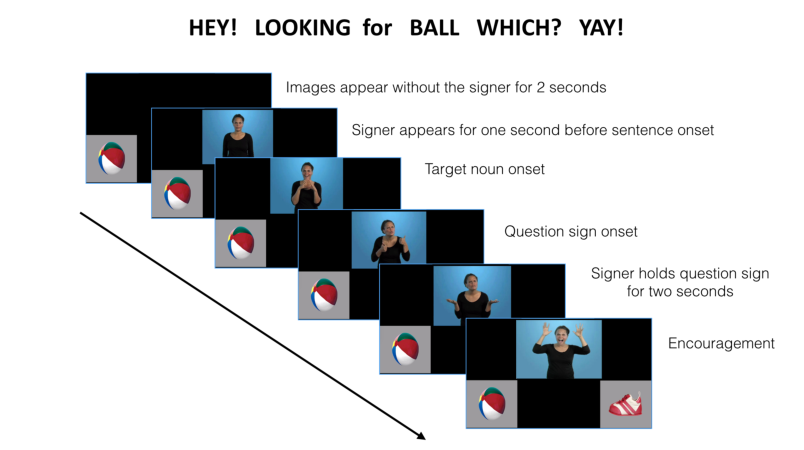
\includegraphics{Figs/timeline-1.pdf}
\caption{Timeline of a trial on the VLP task.}
\end{figure}

\subsubsection{Trial Structure}\label{trial-structure}

Figure 1 shows an example of the stimuli and the timeline of one trial
in the VLP task. On each trial the child saw two images on the screen
for two seconds before the signer appeared. This allowed the child to
inspect both images prior to the start of the sentence. Next, children
saw a still frame of the signer for one second, which gave them the
opportunity to orient to the signer prior to the sentence onset. Each
sentence lasted for approximately five seconds and was followed with a
two second ``hold'' that allowed children to shift away from the signer
to the images on the screen. After the hold, the signer gave neutral,
positive feedback to help maintain the child's focus throughout the
task.

\subsubsection{Linguistic and visual
stimuli}\label{linguistic-and-visual-stimuli}

The linguistic stimuli were designed to be comparable to those used in
previous research and to allow for generalization beyond characteristics
of a specific signer and sentence structure. To accomplish this, ASL
stimuli were recorded by two different native ASL users using two
different but acceptable ASL sentence structures for asking
questions\footnote{See Neidle, MacLaughlin, Lee, Bahan, \& Kegl (1998)
  for a detailed discussion of the acceptability of these two question
  structures. It is important to point out that we first analyzed
  responses for the two sentence frames separately and found no
  significant differences between the two. Thus all analyses we report
  are collapsed across the two sentence structures.}:

\begin{itemize}
\itemsep1pt\parskip0pt\parsep0pt
\item
  Sentence-initial wh-phrase: ``HEY! WHERE {[}target noun{]}?''
\item
  Sentence-final wh-phrase: ``HEY! {[}target noun{]} WHERE?''
\end{itemize}

Before each sentence, the signer used a hand-wave gesture commonly used
in ASL discourse to initiate a linguistic utterance. This served to
shift children's attention away from the images on the screen to the
signer in preparation for the upcoming linguistic information.

Four yoked pairs of eight target nouns (cat---bird, car---book,
bear---doll, ball---shoe) were used. These nouns were selected such that
they would be familiar to most children learning ASL at this age and
have minimal phonological overlap. To prepare the stimuli, two female
native ASL users recorded several tokens of each sentence, matching them
closely in prosody. These candidate stimuli were then digitized,
analyzed, and edited using Final Cut Pro software. The final tokens were
chosen based on naturalness and prosodic comparability. The mean
duration of target nouns was 1134 ms (range = 495-1947 ms). Five filler
trials were interspersed among the 32 test trials (e.g. ``YOU LIKE
PICTURES! MORE WANT?''). Images were digitized pictures presented in
fixed pairs, matched for visual salience with 3--4 tokens of each object
type. Side of target picture was counterbalanced across trials.

\subsubsection{Coding and reliability}\label{coding-and-reliability}

Children's gaze patterns were videotaped and coded frame-by-frame,
yielding a high-resolution record of eye movements aligned with target
noun onset. 25\% of videos were re-coded to assess coder reliability --
agreement within a single frame averaged 98\% on these reliability
assessments.

\subsubsection{Calculating linguistic processing
efficiency}\label{calculating-linguistic-processing-efficiency}

\emph{Accuracy:} Correct looking is a function of the child's tendency
to shift quickly away from the central signer to the target picture in
response to the target sign, and also to remain fixated on the target
picture. To determine the degree to which participants fixated the
appropriate picture across trials, mean proportion looking to target was
calculated for each participant at each 33 ms frame from the onset of
the target noun. Accuracy was defined as the mean proportion of time
spent looking at the target picture out of the total time spent on
either the target picture, the distracter picture, or the signer from
500 to 2000 ms from target noun onset. We selected this window after
looking at the distribution of children's first shifts with the goal of
maximizing the amount of meaningful looking behavior. This window
includes 90\% of children's first shifts off the center signer.
Importantly, the VLP task includes a central signer, which functions as
a central fixation point similar to adult psycholinguistic experiments.
Thus children could produce four different types of responses on a given
trial: (1) signer-to-target shift, (2) signer-to-distractor shift, (3)
signer-to-away shift, (4) no-shift. All four trial types contribute to
accuracy analyses and all 29 children were included.

\emph{Reaction Time:} Reaction time (RT) corresponds to the latency to
shift away from the signer to the target picture, measured from the
onset of the target sign. Incorrect shifts from the signer to the
distractor picture were not included in the computation of mean RT. To
determine whether children's initial shifts were the result of guessing,
we applied a Bayesian latent mixture guessing model implemented in JAGS
(Plummer \& others, 2003). In this model, data are assumed to be
generated by two different processes (guessing and knowledge) which have
different probabilities of success, with the guessing group having a
probability of 0.5 and the knowledge group having a probability greater
than 0.5. The group membership of each participant is a latent variable
that we infer based on their proportion of correct shifts to the target
picture relative to the overall proportion of correct shifts across all
participants (see M. Lee \& Wagenmakers (2013) for a discussion of this
modeling approach). Data from 5 children were excluded because more than
50\% of their posterior mass indicated a guessing strategy with
relatively little uncertainty: posterior probabilities of 0.99, 0.58,
0.97, 0.98, and 0.82 respectively, suggesting that RTs for these
children are not a meaningful measure of their language processing
skill.\footnote{Mean accuracy scores for these participants were: 0.54,
  0.60, 0.42, 0.29, 0.40.} Thus, only signer-to-target shifts for 24
children were included in the RT analyses.

Within children, shifts that occurred prior to 500 ms from noun onset
were excluded because it is likely that these shifts were initiated
before the child had enough time to process sufficient linguistic input
and to mobilize an eye movement; shifts that occurred after 2000 ms were
excluded because these delayed looks are less likely to reflect a
response to the target sign (see Fernald et al. (2001)). In addition,
8\% of trials were excluded because children never shifted off of the
signer. Since children vary in the likelihood that they will shift on a
given trial, mean RTs are based on different numbers of trials across
participants (M = 13.4 trials, range = 3---25).

\section{Results}\label{results}

\begin{figure}[htbp]
\centering
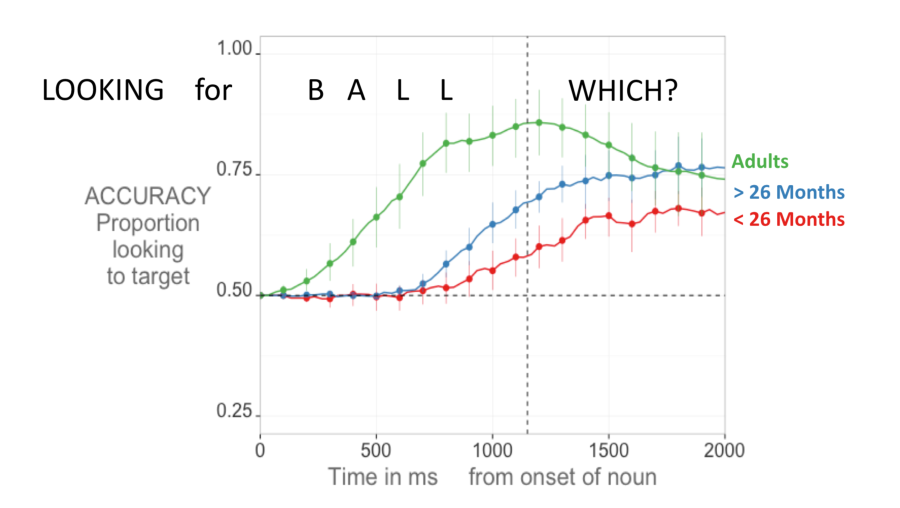
\includegraphics{Figs/profile plot png-1.pdf}
\caption{The timecourse of participants' responses to the target picture
in relation to the unfolding sign for younger children, older children,
and adults. Curves show changes over time in the mean proportion looking
to the correct picture, measured in ms from noun onset; error bars
represent +/- 95\% CI computed by non-parametric bootstrap. The dashed
vertical line indicates mean offset of target nouns (1134 ms).}
\end{figure}

\begin{figure}[htbp]
\centering
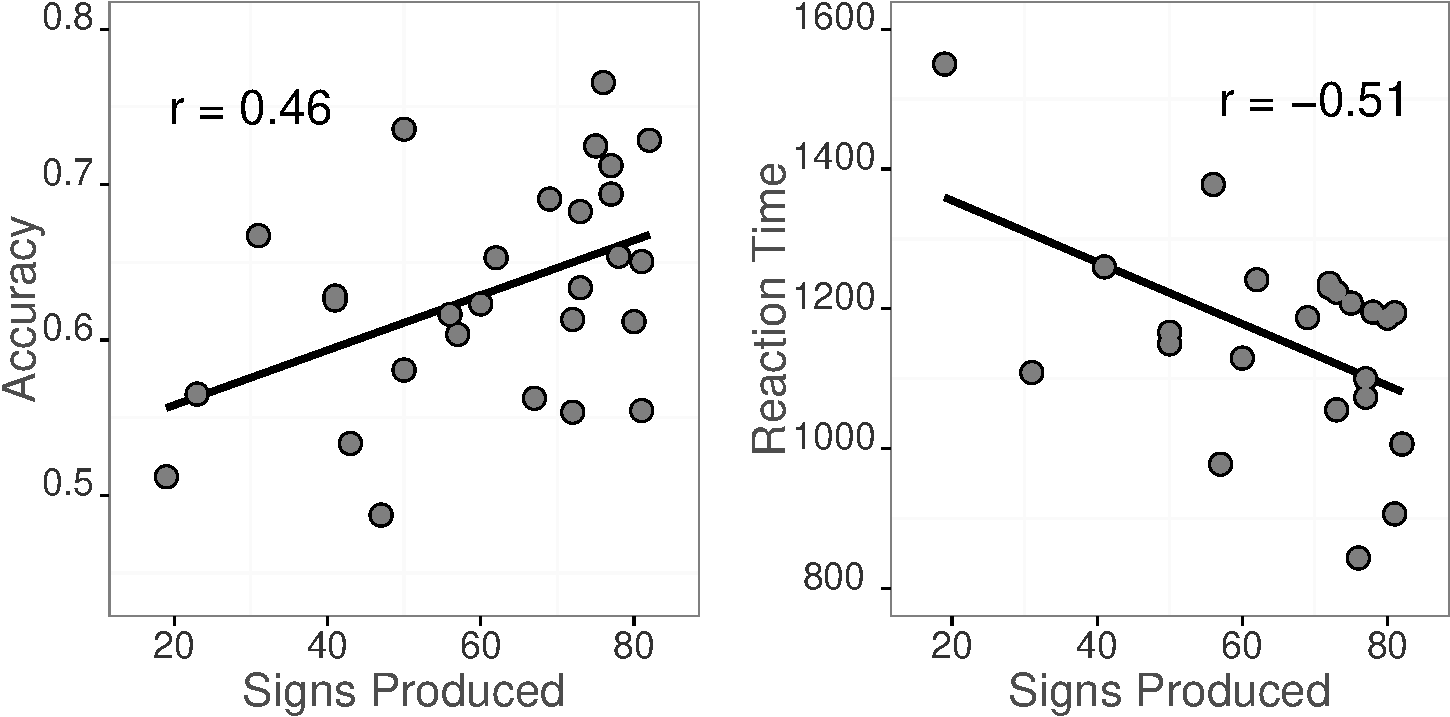
\includegraphics{Figs/vocab scatter plots-1.pdf}
\caption{Relationship between VLP measures and productive ASL
vocabulary. Each data point is an individual child. Panel A shows the
positive relationship between accuracy and vocabulary. Panel B shows the
negative relationship between RT and vocabulary}
\end{figure}

First we present an overview of performance on the VLP task, showing
that children become faster and more accurate at comprehending familiar
signs as they get older and make progress towards adult levels of
language fluency. Then we present analyses of the links between
children's real-time ASL processing skills and both age and productive
ASL vocabulary.

\subsubsection{ASL processing
efficiency}\label{asl-processing-efficiency}

Figure 2 provides an overview of the timecourse of correct orienting to
the referent in response to the target sign. The three curves show
changes in the mean proportion of trials on which participants in each
age group fixated the correct referent at every 33 ms interval as the
target sign unfolded. Before seeing the target sign, all participants
fixated on the signer. Interestingly, both adults and children began to
increase their looking to the target picture before the offset of the
target noun, providing evidence that signers were not waiting until the
end of the linguistic utterance to seek out the target image. Children
were slower to respond and less accurate than adults, maintaining their
gaze on the center signer for approximately 700 ms and reaching a lower
asymptote. The youngest children took longer to orient to the target
(\(Myounger = 1114\) ms, \(Molder = 1224\) ms,
\(t(22) = 1.89, d = 0.23\)) and were less accurate than older children
(\(Myounger = 0.59\), \(Molder = 0.67\), \(t(27) = -3.32, d = 0.36\)).

\subsubsection{Links between processing efficiency and
age}\label{links-between-processing-efficiency-and-age}

Mean accuracy scores, computed over the 500--2000 ms window from noun
onset, were examined as a function of age. Accuracy was strongly
correlated with age (\(r\)(27) = 0.64), indicating that older ASL
learners were more reliable than younger children in fixating the target
picture. Mean reaction times were negatively correlated with age
(\(r\)(22) = -0.38), indicating that older ASL-learning children were
faster to shift to the target picture than younger ones. Mean reaction
times were also negatively correlated with mean accuracy scores
(\(r\)(22) = -0.59) such that those children who were faster to shift to
the target were also more likely to stick on the target image throughout
the analysis window.

Together, the Accuracy and Reaction Time analyses show that signers will
reliably leave a central signer to shift to a target image in the VLP
task, even before the end of the linguistic utterance. Importantly,
signers varied in their response times and accuracy, and this variation
was meaningfully linked to age. Thus, like children learning spoken
language, ASL learners improve their real-time language processing
skills over the second and third years of life, progressing towards
adult levels of language fluency.

\subsubsection{Links between processing efficiency and
vocabulary}\label{links-between-processing-efficiency-and-vocabulary}

Figure 3 shows the relationships between both VLP processing measures
and children's productive ASL vocabulary. Mean accuracy was positively
related to vocabulary size (\(r\)(26) = 0.46) such that children with
higher accuracy scores also had larger productive vocabularies. Mean
reaction times were negatively correlated with vocabulary (\(r\)(21) =
-0.51) indicating that children who were faster to recognize ASL signs
also had larger vocabularies.

It is important to point out that age and vocabulary were strongly
intercorrelated in our sample (\(r\)(21) = 0.72). Multiple regression
analyses indicated that together these factors accounted for
approximately 44.4\% of the variance in accuracy (\(F\)(2, 25) = 10).
Although vocabulary did not contribute significant variance after age
was taken into account (\(r^2\)-change: 3.7\%), age contributed
approximately 23.4\% additional variance beyond vocabulary. Thus, the
majority of the variation in accuracy that was accounted for by age and
vocabulary size was attributable to the shared variance between these
two factors, yet some sources of individual differences in accuracy were
attributable to age above and beyond vocabulary.

Multiple regression analyses also indicated that age and vocabulary
together accounted for approximately 26.1\% of the variance in RT.
However, in contrast to the accuracy measure, neither age nor vocabulary
contributed significant unique variance (\(r^2\)-change: 0.2\%) on the
RT measure. Thus, all of the variation in RT accounted for by age and
vocabulary was attributable to the shared variance between these two
factors.

Taken together, these results indicate that children learning ASL were
more accurate and efficient in identifying the referents of familiar
signs as they got older and developed a larger expressive vocabulary.
These findings are consistent with previous research with children
learning English and Spanish.

\section{Discussion}\label{discussion}

Establishing reference in real-time is a fundamental component of
language learning. To link signs to objects, young ASL users must learn
to resolve an apparent conflict between attending to the source of
linguistic information and shifting their gaze to the surrounding visual
scene. Moreover, they must learn to do this efficiently because language
unfolds rapidly, and if a child does not see a sign, or does not see the
intended referent, the information in that naming event is effectively
unavailable. With this study, we aimed to develop and validate the first
measures of young ASL learners' real-time language comprehension skills
and explore the links between these skills and both age and vocabulary.
There are three main findings from this work.

First, measuring gaze shifts during real-time sentence processing is a
valid way to measure young ASL learners' language development. Previous
work using online measures with adult ASL users has revealed important
aspects of the psycholinguistics of sentence processing. For example,
Lieberman et al. (2014a) showed evidence of real-time activation of
sublexical features of sign and that incremental semantic processing
occurs during real-time sign comprehension. But we did not yet know
whether these online measures would work with very young learners.
Moreover, because gaze serves a variety of functions in ASL, using eye
movements as an index of language comprehension ability might not have
been possible. For example, proficient ASL users rely on vision for: (a)
processing linguistic information, (b) processing the visual world, (c)
regulating turn-taking during conversation (Baker \& Padden, 1978), and
(d) role shifts during narrative production (Bahan \& Supalla, 1995).
However, despite these modality-driven differences, we found that both
adults and children reliably began shifting to the target picture before
the end of the target noun, showing the signature rapid processing
skills thought to be so important for fluent language comprehension. It
is also interesting to consider how the rapid gaze shifts we measured in
the VLP paradigm would compare to the gaze shifting behavior required in
naturalistic interactions to establish mutual gaze to objects (i.e.,
joint attention), which is thought to be critical for early lexical
development (see Lieberman et al. (2014b) for a discussion of joint
attention behavior in ASL).

The second main finding was that, like children learning spoken language
(Fernald et al., 1998), young ASL learners' show measurable age-related
improvement in the efficiency with which they processed language. All of
the target signs were familiar to children in this age range, yet older
children more quickly and accurately identified the correct referent
than younger children. This finding provides additional evidence that
ASL acquisition in native, natural contexts follows a strikingly similar
developmental path to children learning spoken language (Lillo-Martin,
1999; Mayberry \& Squires, 2006). Moreover, this is the first study to
show that real-time ASL \emph{comprehension} skills are linked to early
language development. Prior work on the developmental trajectories of
deaf children has relied on aspects of language production often because
production is easier to see, making it easier to measure. However, a
large amount of research on language acquisition shows that
comprehension often precedes production (see Clark (2009)). Thus, by
developing a fine-grained measure of ASL comprehension, we hope to allow
reserachers and educators to measure children's language skills earlier
in development.

The third result was the discovery of a link between early ASL
processing skills and children's productive ASL vocabularies. We found
that ASL-learning children who knew more signs were also faster and more
accurate in language processing than those who were lexically less
advanced. However, the factors of age and vocabulary size were highly
intercorrelated in this sample and the majority of the associations
between vocabulary and efficiency of language processing were
attributable to variance that was shared between these two factors.
Nevertheless, these results with children learning ASL are consistent
with other studies with English- and Spanish- learning children, which
test a narrower age range and find strong relations between efficiency
in online language comprehension and other concurrent and longitudinal
measures of linguistic achievement (Fernald et al., 2006, 2001; Zangl et
al., 2005). It is important to point out that the direction of the
relationship between vocabulary and processing skills is unclear (for a
detailed discussion see Hurtado, Marchman, \& Fernald (2007)). It could
be that initial differences in processing speed makes it easier for some
children to learn words more quickly. It is also likely that having a
larger vocabulary facilitates sign processing. It might also be the case
that knowing more signs is associated with more efficient
word-recognition skills because lexical growth has led to changes in the
way that lexical forms are represented. Thus, children with larger
vocabularies may be faster and more efficient processors of spoken
language because lexical growth itself has contributed to a shift to
more segmentally-based lexical representations.

In sum, this study provides the first evidence that measuring eye
movements during real-time ASL sentence processing is a valid measure of
age-related changes in young children's visual language comprehension
skills. These findings contribute to the now significant body of
literature highlighting the parallels between signed and spoken language
development when children are exposed to native sign input. We hope that
the development of the VLP task will provide a useful method for
researchers and educators, providing earlier measures of the
developmental trajectories of deaf children, most of whom have much more
heterogeneous and inconsistent language exposure than the ones tested in
the current work.

\section{Acknowledgements}\label{acknowledgements}

We are grateful to the many children and parents who participated in
this research, and to the staff of the California School for the Deaf in
Fremont. Special thanks to Shane Blau, Kat Adams, Melanie Ashland, and
the staff of the Language Learning Lab at Stanford University. This work
was made possible by an NIDCD grant to Anne Fernald and David Corina
(R21 DC012505-1).

\newpage 

\section*{References}\label{references}
\addcontentsline{toc}{section}{References}

Altmann, G. T., \& Kamide, Y. (1999). Incremental interpretation at
verbs: Restricting the domain of subsequent reference. \emph{Cognition},
\emph{73}(3), 247--264.

Anderson, D., \& Reilly, J. (2002). The macArthur communicative
development inventory: Normative data for american sign language.
\emph{Journal of Deaf Studies and Deaf Education}, 83--106.

Bahan, B., \& Supalla, S. (1995). Line segmentation and narrative
structure: A study of eyegaze behavior in american sign language.
\emph{Language, Gesture, and Space}, 171--191.

Baker, C., \& Padden, C. (1978). Focusing on the nonmanual components of
american sign language. \emph{Understanding Language Through Sign
Language Research}, 27--57.

Bellugi, U. (1979). \emph{The signs of language}. Harvard University
Press.

Boudreault, P., \& Mayberry, R. I. (2006). Grammatical processing in
american sign language: Age of first-language acquisition effects in
relation to syntactic structure. \emph{Language and Cognitive
Processes}, \emph{21}(5), 608--635.

Carreiras, M. (2010). Sign language processing. \emph{Language and
Linguistics Compass}, \emph{4}(7), 430--444.

Carreiras, M., Guti{é}rrez-Sigut, E., Baquero, S., \& Corina, D. (2008).
Lexical processing in spanish sign language (lSE). \emph{Journal of
Memory and Language}, \emph{58}(1), 100--122.

Clark, E. V. (2009). \emph{First language acquisition}. Cambridge
University Press.

Corina, D. P., \& Emmorey, K. (1993). Lexical priming in american sign
language. In \emph{34th annual meeting of the psychonomics society}.

Corina, D. P., \& Knapp, H. P. (2006). Lexical retrieval in american
sign language production. \emph{Papers in Laboratory Phonology},
\emph{8}, 213--240.

Dahan, D., \& Tanenhaus, M. K. (2004). Continuous mapping from sound to
meaning in spoken-language comprehension: Immediate effects of
verb-based thematic constraints. \emph{Journal of Experimental
Psychology: Learning, Memory, and Cognition}, \emph{30}(2), 498.

Emmorey, K., \& Corina, D. (1990). Lexical recognition in sign language:
Effects of phonetic structure and morphology. \emph{Perceptual and Motor
Skills}, \emph{71}(3f), 1227--1252.

Fenson, L., Dale, P. S., Reznick, J. S., Bates, E., Thal, D. J.,
Pethick, S. J., \ldots{} Stiles, J. (1994). Variability in early
communicative development. \emph{Monographs of the Society for Research
in Child Development}, i--185.

Fernald, A., \& Marchman, V. A. (2012). Individual differences in
lexical processing at 18 months predict vocabulary growth in typically
developing and late-talking toddlers. \emph{Child Development},
\emph{83}(1), 203--222.

Fernald, A., Perfors, A., \& Marchman, V. A. (2006). Picking up speed in
understanding: Speech processing efficiency and vocabulary growth across
the 2nd year. \emph{Developmental Psychology}, \emph{42}(1), 98.

Fernald, A., Pinto, J. P., Swingley, D., Weinbergy, A., \& McRoberts, G.
W. (1998). Rapid gains in speed of verbal processing by infants in the
2nd year. \emph{Psychological Science}, \emph{9}(3), 228--231.

Fernald, A., Swingley, D., \& Pinto, J. P. (2001). When half a word is
enough: Infants can recognize spoken words using partial phonetic
information. \emph{Child Development}, \emph{72}(4), 1003--1015.

Grosjean, F. (1980). Spoken word recognition processes and the gating
paradigm. \emph{Perception \& Psychophysics}, \emph{28}(4), 267--283.

Harris, M., \& Mohay, H. (1997). Learning to look in the right place: A
comparison of attentional behavior in deaf children with deaf and
hearing mothers. \emph{Journal of Deaf Studies and Deaf Education},
\emph{2}(2), 95--103.

Hildebrandt, U., \& Corina, D. (2002). Phonological similarity in
american sign language. \emph{Language and Cognitive Processes},
\emph{17}(6), 593--612.

Hurtado, N., Marchman, V. A., \& Fernald, A. (2007). Spoken word
recognition by latino children learning spanish as their first language.
\emph{Journal of Child Language}, \emph{34}(02), 227--249.

Hurtado, N., Marchman, V. A., \& Fernald, A. (2008). Does input
influence uptake? Links between maternal talk, processing speed and
vocabulary size in spanish-learning children. \emph{Developmental
Science}, \emph{11}(6), F31--F39.

Lee, M., \& Wagenmakers, E. (2013). Bayesian modeling for cognitive
science: A practical course. \emph{Cambridge UP}.

Lew-Williams, C., \& Fernald, A. (2007). Young children learning spanish
make rapid use of grammatical gender in spoken word recognition.
\emph{Psychological Science}, \emph{18}(3), 193--198.

Lieberman, A. M., Borovsky, A., Hatrak, M., \& Mayberry, R. I. (2014a).
Real-time processing of aSL signs: Delayed first language acquisition
affects organization of the mental lexicon. \emph{Journal of
Experimental Psychology: Learning, Memory, and Cognition}.

Lieberman, A. M., Hatrak, M., \& Mayberry, R. I. (2014b). Learning to
look for language: Development of joint attention in young deaf
children. \emph{Language Learning and Development}, \emph{10}(1),
19--35.

Lillo-Martin, D. (1999). Modality effects and modularity in language
acquisition: The acquisition of american sign language. \emph{Handbook
of Child Language Acquisition}, \emph{531}, 567.

Lillo-Martin, D. (2000). Early and late in language acquisition: Aspects
of the syntax and acquisition of wh-questions in american sign language.
\emph{The Signs of Language Revisited: An Anthology to Honor Ursula
Bellugi and Edward Klima}, 71--90.

Marslen-Wilson, W., \& Zwitserlood, P. (1989). Accessing spoken words:
The importance of word onsets. \emph{Journal of Experimental Psychology:
Human Perception and Performance}, \emph{15}(3), 576.

Mayberry, R. I., \& Eichen, E. B. (1991). The long-lasting advantage of
learning sign language in childhood: Another look at the critical period
for language acquisition. \emph{Journal of Memory and Language},
\emph{30}(4), 486--512.

Mayberry, R. I., \& Fischer, S. D. (1989). Looking through phonological
shape to lexical meaning: The bottleneck of non-native sign language
processing. \emph{Memory \& Cognition}, \emph{17}(6), 740--754.

Mayberry, R. I., \& Squires, B. (2006). Sign language acquisition.

Meier, R. P., Mauk, C., Mirus, G. R., \& Conlin, K. E. (1998). Motoric
constraints on early sign acquisition. \emph{29}, 63--72.

Mitchell, R. E., \& Karchmer, M. A. (2004). Chasing the mythical ten
percent: Parental hearing status of deaf and hard of hearing students in
the united states. \emph{Sign Language Studies}, \emph{4}(2), 138--163.

Neidle, C., MacLaughlin, D., Lee, R. G., Bahan, B., \& Kegl, J. (1998).
Wh-questions in aSL: A case for rightward movement. \emph{American Sign
Language Linguistic Research Project}, \emph{6}.

Newport, E. L. (1990). Maturational constraints on language learning.
\emph{Cognitive Science}, \emph{14}(1), 11--28.

Newport, E. L., \& Meier, R. P. (1985). \emph{The acquisition of
american sign language.} Lawrence Erlbaum Associates, Inc.

Plummer, M., \& others. (2003). JAGS: A program for analysis of bayesian
graphical models using gibbs sampling. In \emph{Proceedings of the 3rd
international workshop on distributed statistical computing} (Vol. 124,
p. 125). Technische Universit at Wien.

Quine, W. (1960). \emph{Word and object}. MIT press.

Snedeker, J., \& Trueswell, J. C. (2004). The developing constraints on
parsing decisions: The role of lexical-biases and referential scenes in
child and adult sentence processing. \emph{Cognitive Psychology},
\emph{49}(3), 238--299.

Tanenhaus, M. K., Spivey-Knowlton, M. J., Eberhard, K. M., \& Sedivy, J.
C. (1995). Integration of visual and linguistic information in spoken
language comprehension. \emph{Science}, \emph{268}(5217), 1632--1634.

Thompson, R., Vinson, D., Fox, N., \& Vigliocco, G. (2013). Is lexical
access driven by temporal order or perceptual salience? Evidence from
british sign language. In \emph{Proceedings of the 35th annual meeting
of the cognitive science society} (pp. 1450--1455).

Waxman, R. P., \& Spencer, P. E. (1997). What mothers do to support
infant visual attention: Sensitivities to age and hearing status.
\emph{Journal of Deaf Studies and Deaf Education}, \emph{2}(2),
104--114.

Zangl, R., \& Fernald, A. (2007). Increasing flexibility in children's
online processing of grammatical and nonce determiners in fluent speech.
\emph{Language Learning and Development}, \emph{3}(3), 199--231.

Zangl, R., Klarman, L., Thal, D., Fernald, A., \& Bates, E. (2005).
Dynamics of word comprehension in infancy: Developments in timing,
accuracy, and resistance to acoustic degradation. \emph{Journal of
Cognition and Development}, \emph{6}(2), 179--208.

\end{document}
